\documentclass[../main]{subfiles}

\begin{document}

\chapter{The Scratch execution model}\label{ch:scratch-execution-model}

%\dictum[J. Maloney, M. Resnick, et al. \\ \textit{The Scratch Programming Language and Environment}]{Concurrency is often considered an advanced programming technique. Yet our everyday world is highly concurrent, so Scratch users
%are not surprised that a sprite can do several things at once.}

Scratch, a popular visual block-based programming language designed for young learners, inherently supports parallel programming.
Each Scratch program (called a project) consists of a number of sprites with individual code (\cref{ch:scratch-the-programming-environment}).
Blocks that are attached together form scripts, and each sprite can have multiple scripts running concurrently as separate threads within the Scratch virtual machine.

The Scratch execution model combines a fixed-step time loop (30 frames per second) with an almost-cooperative threading model.
This means that threads are seldom interrupted, mostly relying on explicit yielding to other threads.
While this approach minimizes the occurrence of race conditions, some concurrency issues persist~\autocite{maloneyScratchProgrammingLanguage2010}.
For instance, the order in which sprites respond to broadcasts can be unpredictable.
Consequently, even without explicit concurrency controls, Scratch is a useful tool for teaching concurrency concepts~\autocite{fatourouTeachingConcurrentProgramming2018}.

However, the current execution model has some drawbacks.
The cooperative nature of the threading model can lead to unexpected behaviour when working with multiple sprites.
Additionally, the execution model complicates the use of debuggers within Scratch.
A traditional step function (which steps one block at a time) exposes execution states that are normally hidden.
Alternative step functions (for example, the one used by Blink, see \cref{subsec:stepwise-execution}) diverge from the normal execution and is thus undesirable.

To address these issues, this chapter begins with an in-depth exploration of Scratch's current execution model.
This analysis is essential for understanding the subsequent section, where we explore the model's shortcomings in more detail.
We then propose some modifications to the execution model, which would solve the issues we have identified.
These modifications are then evaluated to determine their impact on real-world Scratch projects.
Finally, we illustrate that the changed execution model is suitable for use in a Scratch debugger.

\section{Elements of a Scratch program}\label{sec:elements-of-a-scratch-program}

\begin{listing}
    \centering
    \begin{subfigure}{0.45\textwidth}
        \centering
        \begin{scratch}[scale=0.7]
            \blockinit{when \greenflag{} clicked}
            \blockmove{move  \ovalnum{100} steps}
            \blockmove{turn \turnleft{} \ovalnum{90} degrees}
            \blockmove{move  \ovalnum{100} steps}
            \blockmove{turn \turnleft{} \ovalnum{90} degrees}
            \blockmove{move  \ovalnum{100} steps}
            \blockmove{turn \turnleft{} \ovalnum{90} degrees}
            \blockmove{move  \ovalnum{100} steps}
            \blockmove{turn \turnleft{} \ovalnum{90} degrees}
        \end{scratch}
    \end{subfigure}
    \begin{subfigure}{0.45\textwidth}
        \centering
        \begin{scratch}[scale=0.7]
            \blockinit{when \greenflag{} clicked}
            \blockrepeat{repeat \ovalnum{4}}{
                \blockmove{move  \ovalnum{100} steps}
                \blockmove{turn \turnleft{} \ovalnum{90} degrees}
            }
        \end{scratch}
    \end{subfigure}
    \caption{Two Scratch programs that seemingly produce the same result: the sprite moves in a square of 100 steps, and finally stops at the same position as the start of the progam.}
    \label{lst:scratch-two-programs}
\end{listing}

A Scratch program consists of zero or more sprites and a stage (see also \cref{ch:scratch-the-programming-environment}).
Together, the sprites and stages are called targets (since they are drawn on the screen).
All sprites have their own local state: the variables and visual properties of the sprite (e.g.\ position, size, bounding box, colour, direction).
Clones are also targets: they are drawn, but share their code with their original sprite (but they do have some state, like the visual properties).
In the virtual machine, there is no substantial difference between how targets (sprites, stage, clones) are handled, so we can just consider targets for the remainder of this chapter.

Code-wise, the Scratch blocks are organized into categories (see \cref{subsec:using-the-environment-and-the-blocks}).
However, in this case, it is useful to look at their technical type, which corresponds to their shape.
In total, there are seven types of blocks:

\begin{enumerate}[noitemsep]
    \item Hat blocks \scratchinline{\blockinit{\hspace{1em}\dots\hspace*{1em}}}, which are placed at the start of a script (they are named hat blocks since they visually sit on top of a script).
        A script can only have one hat block.
        They function as event listeners, which trigger execution of the script if the event occurs.
    \item Stack blocks \scratchinline{\blockmove{\hspace{1em}\dots\hspace*{0.5cm}}}, representing program statements.
        These are the most common blocks.
        They are called stack blocks since they are stacked on top of each other.
        Stack blocks broadly fulfil the role of statements in Scratch.
    \item C blocks \scratchinline{\blockif{\hspace{1em}\dots\hspace*{1em}}{\blockspace[0.2]}}, which are named after their shape.
        They are used for most of the control flow blocks: loops and branches.
        The variant for the if/else block is sometimes named an E block, since it has two slots.
    \item Reporter blocks \setscratch{baseline=c,scale=0.5}\ovalmove{\hspace{1em}\dots\hspace*{1em}}, act as variables or values and can be slotted into other blocks.
        Operators that result in a value also have this shape.
        The reporter blocks fulfil the role of expressions.
    \item Boolean blocks \setscratch{baseline=c,scale=0.5}\boolsensing{\hspace{1em}\dots\hspace*{1em}}, which are analogous to reporter blocks, but result in a boolean.
    \item Cap blocks \scratchinline{\blockstop{\hspace{1em}\dots\hspace*{1em}}}, which end a script: no blocks can be added afterwards.
        Note that the infinite loop block, for example, is both a C block and a cap block.
    \item Custom blocks \scratchinline{\initmoreblocks{define\hspace{1em}\dots\hspace*{1em}}}, which define ``procedures''.
\end{enumerate}

\section{Related work}\label{sec:execution-related-work}

The Scratch execution model is defined by its implementation in the virtual machine.
There exists, at least to the knowledge of the authors, no comprehensive formal description of the execution model.
This does not mean there is no prior work.
From the Scratch team, \textcite{maloneyScratchProgrammingLanguage2010} provide a high-level description of the threading model.

Another body of works that provides insights into the Scratch execution model comes from the \emph{Chair of Software Engineering II} group, led by Prof.\ Dr.\ Gordon Fraser.
These publications all provide descriptions for parts of the execution model.

First, \textcite{stahlbauerTestingScratchPrograms2019} propose a formalization of three aspects in Scratch: the user perspective, a syntactic model and a semantic model.
They describe the semantics of Scratch with a memory model based on message passing.
Next, \textcite{stahlbauerVerifiedScratchProgram2020} develop LeILa, an intermediate language to which Scratch projects can be translated, with an intended use of performing analysis on Scratch projects.
The authors also provide a formalization of LeILa, but use approximations in some areas.
Also, \textcite{gotzModelbasedTestingScratch2022} model the state-based behaviour of Scratch programs using a finite state machine.
Finally, \textcite{deinerAutomatedTestGeneration2023} delve deeper into the actual execution of the virtual machine, while also proposing some modifications to it, for example, to make execution deterministic.

Other block-based languages also have to deal with concurrency.
For example, MakeCode also uses a non-preemptive threading model, inspired by the Scratch~\autocite{ballMicrosoftMakeCodeEmbedded2019}.
There has also been some work on concurrency and concurrency controls in other block-based languages~\autocite{chungConCodeItComparisonConcurrency2020}.
However, since most of these languages do not use the Scratch virtual machine for execution, their applicability is limited.

\section{The current execution model}\label{sec:the-current-execution-model}

\subsection{Execution of a Scratch program}\label{subsec:execution-of-a-scratch-program}

\marginnote{Arguably, it is more of a concrete syntax tree, as e.g. the position of blocks is also saved. However, in Scratch's case, the differences are minimal, so we call it an abstract syntax tree, as Scratch themselves do.}
When executing Scratch code, the virtual machine transforms the blocks into an abstract syntax tree.
These are organized by target, and every script of every target results in a thread inside the virtual machine.
These are green threads: implemented fully in the virtual machine.

The virtual machine is thus responsible for scheduling these threads.
A schematic overview of the interaction between the different parts is \cref{fig:blink-architecture}.
It uses an almost-cooperative threading model, which \textcite{maloneyScratchProgrammingLanguage2010} call the ``Scratch threading model''.
This means it is mostly non-preemptive: the virtual machine will not interrupt threads at arbitrary points in their execution.
The threads must voluntarily yield control, or reach a limited set of points in their execution.
The rational is given in~\cite{maloneyScratchProgrammingLanguage2010}: ``Scratch builds concurrency control into its threading model in a way that avoids most race conditions, so that users do not need to think about these issues.
This is done by constraining where thread switches can occur.''.

At four well-defined points, a thread always yields, thus causing said thread switching:
\begin{enumerate}
    \item When a block is executed that has a fixed duration.
        There are a number of blocks that fall under this category.
        \scratchinline{\blockcontrol{wait \ovalnum{}}} is an obvious inclusion, but this also applies to \scratchinline{\blockmove{glide \ovalnum{} secs to x: \ovalnum{} y: \ovalnum{}}}, for example.
        \scratchinline{\blocksound{play sound \ovalsound*{} until done}} also falls under this category, even if there is no explicit time.
    \item When a block waits on execution of other blocks.
        For example, \scratchinline{\blockevent{broadcast \selectmenu{something} and wait}}.
    \item The last block of a loop (thus \scratchinline{\blockinfloop{forever}{\blockspace[0.2]}}, \scratchinline{\blockrepeat{repeat \ovalnum{}}{\blockspace[0.2]}}, and \scratchinline{\blockrepeat{repeat until \boolempty[1em]{}}{\blockspace[0.2]}}).
        This means thread switching will occur after every loop iteration.
    \item A recursive procedure call is detected.
        Scratch attempts to detect these (up to five levels of indirection) and will yield the thread on each call if it detects a recursive call.
\end{enumerate}

There is one exception: when using procedures ``without screen refresh'', Scratch will interrupt a thread that runs longer than \qty{500}{\milli\second}.
This is called the ``wrap timer'', and has some curious edge cases\footnote{\url{https://github.com/scratchfoundation/scratch-vm/issues/2834}}.

The threads are executed in a first-come, first-serve manner: there are no priorities nor changes in thread order.
The first thread is executed until it yields or ends, then the next thread, and so on.
We call the execution within one thread until it yields or ends a \term{turn}.
A thread can have one of three conceptual states: \emph{done}, \emph{running}, and \emph{yield}.

\begin{figure}
    \centering
    \includestandalone{scratch-model}
    \caption{Overview of the interplay between the threading model and the ``game loop''. Within one step (which is done 30 times per second), one or more ticks are executed. The arrow with \CircledText{2} illustrates this: after the first tick, another is started if less than \qty{75}{\percent} of the step time (the time one step has to complete, \qty{33}{\milli\second}) has been used, and a redraw has not been requested, and Scratch is not in turbo mode. Within one tick, a turn is executed for each thread \CircledText{1}: a thread executes until it terminates or the thread yields.}
    \label{fig:scratch-model-explained}
\end{figure}

\marginnote{Scratch 3 should actually run at 60 FPS; however Scratch enables a compatibility mode by default, resulting in 30 FPS.}
The virtual machine uses a \emph{fixed-time step with synchronization} main loop~\autocite{nystromGameProgrammingPatterns2014}, also called a \emph{synchronized coupled model}~\autocite{valenteRealTimeGame2005}.
This means that the virtual machine runs in \term{steps}: internally, the \texttt{step} function is called every \qty{33}{\milli\second} (so 30 times a second, commonly known as 30 frames per second).

In each step, the virtual machine will execute one or more ticks.
A \term{tick} is one turn in every thread: the first thread is executed until it yields or terminates, then the second thread and so on.
After the tick, a redraw is performed if needed (in practice this is always done, as the source code contains a to-do to implement selective redrawing).
After the first tick is finished, the virtual machine decides whether to run another tick (\cref{fig:scratch-model-explained}).
A new tick is started if less than \qty{75}{\percent} of the step time (the time one step has to complete, \qty{33}{\milli\second}) has been used and a redraw has not been requested.
Note that once a tick has started, it is run completely and cannot be stopped.
The arbitrary \qty{75}{\percent} is intended to prevent frame drops: steps that take longer than their allocated step time, meaning the next step is delayed.
Also, in practice, many blocks request a redraw, so in many Scratch projects, a step only ever runs one tick.

\begin{figure}
    \centering
    \begin{subfigure}{0.40\textwidth}
        \includestandalone{threading-no-loop}
    \end{subfigure}
    \begin{subfigure}{0.59\textwidth}
        \includestandalone{threading-with-loop}
    \end{subfigure}
    \caption{The execution of the two programs from \cref{lst:scratch-two-programs}. In the unrolled version (left), all code is executed in the first turn, meaning only one tick and step is needed. In the version with loop (right), the loop yields after each iteration, meaning the rest of the step is filled with idle time. In total, four steps are needed. }
    \label{fig:scratch-two-execution}
\end{figure}

A concrete example of the execution model is given by \cref{fig:scratch-two-execution}, which shows the execution of the programs of \cref{lst:scratch-two-programs}.
These programs have only one thread.
Since none of the blocks in the unrolled program yield the thread, the full program is executed in one step.
In the other version, with a loop, the thread yields after each iteration of the loop, meaning the program needs four steps.
This does result in an observable difference: in the unrolled program, the sprite does not move visually.
As a redraw only happens between steps, the sprite is back at its original position.
In the looped version, the sprite moves four times (albeit very fast), as there is a redraw between each step.

\subsection{Implementation details}\label{subsec:implementation-details}

How different parts of the virtual machine implement the execution model from \cref{subsec:execution-of-a-scratch-program} is shown in \cref{fig:blink-architecture}.
When the user interface loads a project, it also starts the virtual machine.
This means that the game loop is active (this is done in the class \texttt{Runtime}).

New threads are only created in two scenarios:
\begin{itemize}[noitemsep]
    \item Code needs to be executed, either because an event triggered some hat blocks (green flag, key press, etc.) or because the user clicked on some blocks.
    \item When ``stage monitors'' or watchers are active.
        These are used in the user interface to show the value of variables or properties.
        The watchers for variables also allow the user to change the value of the variable.
\end{itemize}

The \texttt{Runtime} calls the method \mintinline{javascript}{stepThreads} in the \texttt{Sequencer} class.
This class is responsible for implementing the ticks.
After each tick, done threads are removed, and a new tick is started if possible.
It is also here that the thread status is managed.
While there are three conceptual statuses, the implementation has five:
\begin{description}[noitemsep]
    \item[\texttt{done}] The thread has finished executing all blocks and will be removed after this tick.
    \item[\texttt{running}] The thread is being executed and has more blocks to execute.
        It will be scheduled again next tick.
    \item[\texttt{yield}] The thread is waiting an amount of time.
        The thread is scheduled again next tick to see if the wait time is over.
    \item[\texttt{promise wait}] The thread is waiting for a JavaScript promise to be resolved, after which the thread will be set to \texttt{running}.
    \item[\texttt{yield tick}] The thread yields until the next step.
        The purpose of this status seems to be some performance optimizations to aid with benchmarking\footnote{\url{https://github.com/scratchfoundation/scratch-vm/pull/1211}}.
\end{description}

Each thread maintains a stack structure.
The \texttt{Sequencer} will then look up the next block on said stack, and if there is one, it will call the \texttt{Execute} class.
That class will actually execute the block on the stack.
For normal blocks (confusingly called ``stack blocks'', since they stack in a script), the current block is popped from the stack, the block is executed, and the next block is put on the stack.
The stack is only useful when working with C-blocks or procedures.
For example, C blocks will push the first block in their slot on the stack.
In the case of a loop, a counter is saved in the stack frame to determine how many times the loop should be run.
The exact implementation of the stack is less relevant for this chapter, so it is left to the reader to browser the source code.

\section{Limitations of the execution model}\label{sec:limitations-of-the-execution-model-for-the-debugger}

This section illustrates a few limitations of the current execution model, first in general and then specifically for a debugger.

\subsection{In general}\label{subsec:in-general}

\begin{listing}
    \centering
    \begin{scratch}[scale=0.6]
        \blockinit{when \greenflag{} clicked}
        \blockmove{go to x: \ovalnum{0} y: \ovalnum{112}}
        \blockpen{erase all}
        \blockpen{set pen color to \pencolor{ppcolor}}
        \blockpen{set pen size to \ovalnum{5}}
        \blockpen{pen down}
        \blockmove{point in direction \ovalnum{108}}
        \blockrepeat{repeat \ovalnum{4}}{
            \blockmove{move \ovalnum{80} steps}
            \blockmove{turn \turnright{} \ovalnum{36} degrees}
            \blockmove{move \ovalnum{80} steps}
            \blockmove{turn \turnright{} \ovalnum{36} degrees}
        }
        \blockpen{pen up}
    \end{scratch}
    \hspace{3em}
    \begin{scratch}[scale=0.6]
        \blockinit{when \greenflag{} clicked}
        \blockinfloop{forever}{
            \blockif{if \boolsensing{touching color \pencolor{blue}} then}{
                \blockstop{stop \selectmenu{all}}
            }
        }
    \end{scratch}
    \caption{The implementation, with a bug in the first script (left) and a non-working second script (right).}
    \label{lst:star-model-implementation}
\end{listing}

\begin{figure}
    \begin{subfigure}{0.45\textwidth}
        
\includegraphics[width=\textwidth]{star-before}
        \caption{The stage before execution.}
        \label{fig:star-exercise-model-before}
    \end{subfigure}
    \hfill
    \begin{subfigure}{0.45\textwidth}
        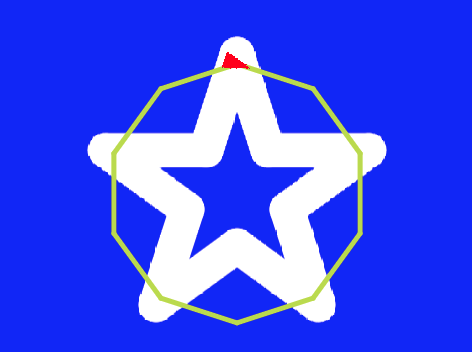
\includegraphics[width=\textwidth]{star-after}
        \caption{The stage after execution.}
        \label{fig:star-exercise-model-after}
    \end{subfigure}
    \caption{Result of running the implementation from \cref{lst:star-model-implementation} for the \emph{Star} exercise.}
    \label{fig:star-exercise-model}
\end{figure}

As \textcite{maloneyScratchProgrammingLanguage2010} mentioned, the Scratch threading model does not solve all issues with concurrency.
To illustrate this point, we will consider a variant on the \emph{Star} exercise from \cref{subsec:star-exercise}.
In this exercise, the goal is to let a sprite move around on a path without falling into the water (read touching a blue colour.)
\Cref{lst:star-model-implementation} shows an implementation for this exercise with an additional script that will stop execution if the sprite touches something blue.
We asked a number of educators that had experience with Scratch to predict the behaviour of this implementation.
All of them expected to execution to stop either when the sprite first touches the water or after the block when the sprite first touches the water.
However, as can be seen in \cref{fig:star-exercise-model-before,fig:star-exercise-model-after}, where the canvas is shown before and after running the code, the second script that should have stopped execution did not work.

The reason for this is the non-preemptive thread switching: the body of the loop is always executed atomically.
At the start of the loop, the sprite does not touch the water.
After execution of one iteration, the sprite is back on the path and does not touch the water.
Therefore, whenever the second script is executed, the sprite is not touching the water, which explains why the execution was not stopped.

Consider the original code in the \emph{Star} exercise from \cref{subsec:star-exercise}.
The second script there does not stop the execution, but uses Blink's pause block to halt the execution.
Using the current execution model, the pause block will not function for the same reasons mentioned above.

\subsection{Specifically for a debugger}\label{subsec:specifically-for-a-debugger}

A fundamental feature of any debugger is the ability to step through code: executing one statement and then pausing the execution to facilitate inspection of the program state.
The functionality is also essential in debuggers for Scratch: all existing debuggers for Scratch implement it.
In Scratch, executing a single statement translates to executing a single block.

However, the traditional single-block stepping has some drawbacks in Scratch.
A first drawback is that users have to click a lot, since the stepping functionality is global, not per thread.
Secondly, and more importantly, the step functionality exposes details of the Scratch execution model to the users.
For example, thread switching, which is normally implicit in Scratch's perceived parallel execution, becomes visible to the users during debugging.

Additionally, debuggers must choose what to do with intermediate states that are typically hidden during normal execution.
For instance, five consecutive blocks would result in one redraw in the normal execution.
One choice is to not alter the redraw logic (thus only redrawing when the normal execution would redraw), but this results in steps having no visual impact, even if the block changes the visuals.
The other choice is to redraw after every step.
While the effect of every block (and step) is then visible, this exposes intermediary steps that would normally not be drawn.
Some blocks (for example, checking if a sprite touches a colour) use the visual state, meaning these additional redraws can result in a different execution of the project.

As described in \cref{sec:blink-software-architecture}, our debugger Blink takes a different approach to the stepping feature.
We believe it is useful to maintain the observed parallelism of Scratch in the debugger: we define a step in the debugger as executing one block in every thread.
This approach allows users to keep focus on relevant threads without distractions from thread switches, which can be cumbersome in complex programs.
Users can thus focus on the script(s) they believe are involved in the failure while ignoring (correct) scripts running at the same time.

This approach does come at a price: it changes the Scratch execution model, which is not trivial due to two main considerations:

\begin{enumerate}
    \item If the execution model is only changed when debugging, the debugger does not debug the same program as when running the program.
        This can result in different behaviour, meaning the bugs for which the debugger is used are no longer present or new bugs, unique to the debugger, could be introduced.
    \item If the execution model is changed, we need to ensure that existing Scratch programs keep working and that we do not introduce concurrency problems, as the current execution model of Scratch was explicitly chosen to avoid those.
\end{enumerate}

We opt for the second option: modifying the Scratch execution model.
In the next section, we discuss what we changed, after which we investigate if existing Scratch projects can continue to work.

\section{New execution model}\label{sec:a-family-of-new-execution-models}

In line with how we want the stepping feature of the debugger to work, we have decided to change the Scratch execution model as follows: we modify a turn to execute exactly one block before yielding.
Thus, in a single tick, the virtual machine will execute a single block in every thread.

As there is often only one tick per step (due to many blocks requesting redraws), this means that only one block would be executed per step (thus one block for every thread per \qty{33}{\milli\second}).
The consequence is that this makes execution much slower than in the original execution model.

A possible solution is to modify the number of steps that are taken.
For example, it might be better to run at twice or more times the number of steps per second.
In turbo mode, this would mean the steps are done as fast as the hardware allows.
While this does make everything go much faster, it does introduce a big difference in execution time between a performant machine and a slower machine.

These changes to the execution model have as a benefit that the \emph{Star} exercise will work as intended (\cref{fig:scratch-two-execution}).
Since the first thread will yield after the first block in the loop, the exercise will work as intended.
It can also illustrate that this does introduce concurrency considerations that were not present in the original execution model.
For example, if the conditional block in the second thread evaluates to true, the first thread will execute another block before execution is stopped by the block inside the conditional block from thread two.

In the next sections, we analyse existing Scratch projects to determine which number of steps that most closely results in the same execution speed as the original execution model.
We also take this opportunity to analyse the complexity and block use in Scratch projects, to evaluate whether the concurrency considerations would cause problems.

\section{Exploration of Scratch projects}\label{sec:evaluation-of-scratch-projects}

As Scratch is used by many students, it is important that changes to the execution model do not adversely affect existing Scratch projects.
However, this requires us knowing what Scratch projects look like.
The aim of this analysis is to determine what blocks are used in Scratch projects, how big projects are, and what programming concepts are used.

We begin by looking at existing work on analysing Scratch projects, followed by our own analysis.

\subsection{Existing analyses}\label{subsec:existing-analyses}

\makenote*{There is some discussion if the cyclomatic complexity is a useful metric. It might have no more predictive ability than lines of code \autocite{hattonInvitedTalkRole2008,fentonCritiqueSoftwareDefect1999,cherfInvestigationMaintenanceSupport1992}.}
\Textcite{aivaloglouHowKidsCode2016} analysed \num{250000} Scratch 2.0 projects that they scraped from the public Scratch site.
They looked at the types of blocks used, the size of the projects, and the complexity.
For the complexity, they utilize the cyclomatic complexity metric~\autocite{mccabeComplexityMeasure1976}.
The considered decision points are the \texttt{if} and \texttt{if-else} blocks.

They found that most Scratch projects are small: \qty{75}{\percent} have less than 5 sprites, 12 scripts, and 76 blocks.
\qty{25}{\percent} has less than 12 blocks, although there are some huge projects with more than \num{20000} blocks.
They also found that about \qty{78}{\percent} of projects have no decision points.

\Textcite{fronzaApproachEvaluateComplexity2020} investigate Scratch projects with different complexity metrics.
The dataset is, however, much more limited: 80 projects were analysed.
\makenote*{The validity of the Halstead metrics is even more controversial~\autocite{hamerHalsteadSoftwareScience1982,shenSoftwareScienceRevisited1983,jonesDimensionalAnalysisHalstead2019}.}
The authors also measure the cyclomatic complexity, in addition to some Halstead complexity measures~\autocite{halsteadElementsSoftwareScience1977}, and their own proposal for a ``when'' metric.
They do use more decision points for the cyclomatic complexity (\texttt{if}, \texttt{if-else}, \texttt{repeat until}, \texttt{wait until}, \texttt{and}, \texttt{or}).
The proposed ``when'' metric counts the number of ``when'' blocks (e.g.\ hat blocks with certain conditions).

\subsection{A new dataset of Scratch projects}\label{subsec:a-new-dataset-of-scratch-projects}

Since the dataset for \textcite{aivaloglouHowKidsCode2016} consists of Scratch 2.0 projects and \textcite{fronzaApproachEvaluateComplexity2020} only analyse 80 projects, we found it necessary to collect a new dataset of Scratch projects.

To create a new dataset, we used the Scratch API\footnote{\url{https://en.scratch-wiki.info/wiki/Scratch_API}} as follows.
Creating a new project provided an identifier, which we used as a starting point.
We then subtract one from the identifier, downloaded the project if possible, and continued.

This resulted in \num{237926} projects.
From those, \num{207} were corrupt or for an older version of Scratch.
We also filtered out the following projects: \num{37936} (\qty{15.9}{\percent}) were empty and \num{4411} (\qty{1.9}{\percent}) had no executable code (e.g.\ only head blocks or scripts without head blocks).
This results in a final dataset of \num{195372} Scratch projects we considered for further analysis.

\subsection{Analysing Scratch 3.0 projects}\label{subsec:analysing-scratch-3.0-projects}

Hairball~\autocite{boeHairballLintinspiredStatic2013} is commonly used to analyse Scratch projects (it is also used by the existing analyses), but does not support Scratch 3.0 projects.
% \footnote{TODO: url to repo}
For this reason, we have implemented a very similar piece of software in JavaScript.
It also supports plugins to support extensions for other analyses.
Being written in JavaScript, it has the advantage that it can reuse parts of the Scratch virtual machine, like reading and parsing Scratch projects.

Wherever possible, we have used the same definitions and metrics as used by \textcite{aivaloglouHowKidsCode2016}, for ease of comparison.

\subsection{Use of blocks}\label{subsec:use-of-blocks}

Scratch blocks can be categorized into seven types, based on their shape (\cref{sec:elements-of-a-scratch-program}).
\Cref{fig:block-shapes} shows their usage.
Blocks can also be put into categories (\cref{subsec:using-the-environment-and-the-blocks}).
The number of projects that use a block from a certain category is shown in \cref{fig:block-categories}.
Note that these numbers do not fully compare with \textcite{aivaloglouHowKidsCode2016}: since then, some new Scratch extensions were added, and the pen-related blocks have moved to an extension.

\begin{figure}
    \centering
    \includestandalone{block-shapes}
    \caption{
        Number of blocks by shape in all projects.
        The total number of blocks is \num{47808628}.
        Note that the \textit{forever} block is counted twice (as a cap block and a C block), and procedure-defining blocks are counted as hat blocks.
    }
    \label{fig:block-shapes}
\end{figure}

\begin{figure}
    \centering
    \includestandalone{block-categories}
    \caption{
        Number of projects that use blocks from a certain category.
        Excluded are custom blocks, and all blocks for extensions are counted together.
    }
    \label{fig:block-categories}
\end{figure}

By looking at the blocks, we see the first indication that most projects are small: \qty{17.0}{\percent} of projects only use hat and stack blocks, and \qty{19.5}{\percent} of projects use no C blocks.

We can also see that extensions are not used that much.
Only \qty{12.2}{\percent} of projects use any extension.
The Pen extension is the most popular one, appearing in \qty{6.9}{\percent} of projects.

\subsection{Size and complexity}\label{subsec:size-and-complexity}

\begin{table}
    \centering
    \caption{
        Size and complexity statistics about the \num{195372} non-empty Scratch projects in our dataset.
        Unless otherwise noted, all numbers are shown per project and blocks are counted as logical lines of code.
        The numbers shown in order are the mean and the five-number summary: the minimum, the first quartile, the second quartile (the median), the third quartile, and the maximum.
    }
    \label{tab:loc-scratch}
    \addfontfeatures{Numbers={Monospaced,Lining}}
    \begin{tabular}{|l|S|S[table-format=2.0]|S[table-format=2.0]|S[table-format=2.0]|S[table-format=2.0]|S[table-format=5.0]|}
        \hline
        {} & {mean} & {min} & {Q1} & {Q2} & {Q3} & {max} \\
        \hline
        sprites (with code) & 4.98 & 1 & 1 & 2 & 5 & 1000 \\
        scripts (with code) & 19.73 & 1 & 2 & 4 & 11 & 9134 \\
        \hline
        blocks (logical lines) & 203.14 & 2 & 9 & 22 & 75 & 24084 \\
        blocks (physical lines) & 150.81 & 2 & 8 & 20 & 65 & 20249 \\
        dead blocks & 42.25 & 0 & 0 & 0 & 3 & 14912 \\
        \hline
        blocks per script & 10.30 & 1 & 2 & 5 & 10 & 5497 \\
        \hline
        \shortstack[l]{cyclomatic complexity \\ per script} & 1.85 & 1 & 1 & 1 & 2 & 5497 \\
        \hline
    \end{tabular}
\end{table}

\Cref{tab:loc-scratch} shows a summary of the project size for our dataset.
In the rest of this subsection, we detail some choices we made in analysing the projects and draw some conclusions.

When considering the size of a program, a frequently used metric is lines of code.
However, there is no universal agreed upon manner in which to count lines of code~\autocite{nguyenSLOCCountingStandard2007}.
Two variants are frequently used: physical lines of code (the number of lines in the source files) and logical lines of code (an approximation of the number of statements or expressions).
While normally counting the physical lines of code is easy and counting logical lines requires some consideration, the reverse is true in Scratch.
For counting logical lines of code, we can simply count all blocks.
For physical lines of code, we chose to count the number of ``main'' blocks in a script.
This means we do not count blocks used as arguments, e.g.\ the condition of a loop block is not counted.

When counting the number of scripts per project, we excluded scripts that consist only of one or more hat blocks, as these do nothing.
We similarly excluded sprites without code from the count of sprites per project.

From these data, we can conclude that \qty{75}{\percent} of projects have less than 5 sprites, 11 scripts, and 80 blocks.
\Textcite{aivaloglouHowKidsCode2016} found that this was 5 sprites, 12 scripts, and 76 blocks, which are highly similar findings.
We can conclude that most Scratch projects are small.

\begin{figure}
    \begin{wide}
        \includestandalone[width=\linewidth]{cyclomatic-complexity}
    \end{wide}
    \caption{
        The distribution of the scripts based on their cyclomatic complexity.
        Scripts with complexities higher than 10 have been bundled into the last bucket.
    }
    \label{fig:scratch-cc}
\end{figure}


For the cyclomatic complexity, we used the same decision points as \textcite{aivaloglouHowKidsCode2016}.
\Cref{fig:scratch-cc} shows the distribution of the cyclomatic complexity in the Scratch projects.
Our findings are again similar to what \textcite{aivaloglouHowKidsCode2016} found: most scripts (\qty{72.6}{\percent}) do not contain any decision points.
Additionally, another \qty{15.3}{\percent} has just one decision point.
On the other end of the spectrum, \qty{1.6}{\percent} has a complexity larger than 10, and 667 scripts (\qty{0.00017}{\percent}) have a complexity larger than 100.

In summary, most projects are small (\qty{75}{\percent} has less than 5 sprites, 11 scripts, and 80 blocks), and most scripts (\qty{72.6}{\percent}) have no decision points.

\subsection{Programming concepts}\label{subsec:programming-concepts}

\begin{table}
    \centering
    \caption{Prevalence of programming concepts in Scratch projects.}
    \label{tab:scratch-programming-concepts}
    \begin{tabular}{|l|S[table-format=6.0]|S|}
        \hline
        {Concept} & {№ of projects} & {№ of scripts (\%)} \\
        \hline
        User input blocks & 90703 & 46.43 \\
        Random & 67403 & 34.50 \\
        \hline
        Conditional statements & 80664 & 41.29 \\
        Loop statements & 151050 & 77.31 \\
        Repeat with condition & 28526 & 14.60 \\
        \hline
        Variables & 67526 & 34.56 \\
        Lists & 18331 & 9.38 \\
        \hline
        Procedures & 33319 & 17.05 \\
        \hline
    \end{tabular}
\end{table}

\Cref{tab:scratch-programming-concepts} is an overview of the prevalence of some programming concepts in the analysed Scratch projects.
While the number of projects that use procedures (\qty{17.1}{\percent}) is higher than what was found by \textcite{aivaloglouHowKidsCode2016}, it is still not used that much: a majority of projects do not use it.
Most projects do use loop statements (\qty{77.3}{\percent}), the number of projects using a conditional loop is much smaller (\qty{14.6}{\percent}).
Less than half of projects use conditional statements, and less than half use user input blocks.
About a third (\qty{34.56}{\percent}) of projects use variables, and only \qty{9.38}{\percent} uses lists.
This means that large numbers of projects are simple (and this is what we would expect, given that previous metrics on project size).

\section{Evaluation of the new execution model}\label{sec:evaluation-of-the-new-execution-model}

TODO: benchmark

\section{Impact for debuggers and conclusion}\label{sec:conclusion}

In \cref{ch:blink}, we proposed a debugger for Scratch with a non-traditional step method.
Instead of stepping a single block at a time, we want to step a single block in every thread of a Scratch program (thus in every script).
However, this introduces two downsides:
\begin{enumerate*}[label=\emph{\roman*})]
    \item the step function exposes internal program state that is normally not visible to the users, and
    \item the debugger uses a different execution model as regular execution, but a debugger should deviate from normal execution as little as possible
\end{enumerate*}.

This chapter then asks if we can modify the execution model of Scratch in such a way that the step functionality of a debugger is possible and that the changed execution model is usable for normal execution.
To this end, we first take a detailed look at the existing execution model, due to a lack of existing literature on the topic.
This model is the result of multiple years of work in the Scratch virtual machine and contains many nuances.
The current execution model has been chosen to avoid race conditions, but does not avoid all concurrency-related issues: there are some surprising consequences of the threading model in particular.

Any changes to the execution model must not have adverse consequences for existing Scratch projects.
When then analyse how Scratch is used, by replicating select metrics of previous investigations into what Scratch projects look like.
\Textcite{aivaloglouHowKidsCode2016} did a previous analysis for Scratch 2.0 projects.
The results for Scratch 3.0 projects are broadly similar: most Scratch projects are small and simple, but there are a few big and complex ones.

Finally, we benchmark the changes to the execution model on a selection of projects, informed by our previous analysis.
While there are differences in behaviour for Scratch projects, we believe these to be acceptable.
The modified execution model is thus suitable for our stepping methode for debuggers and reducing concurrency-related surprising behaviour, while not adversely affecting existing projects.

We also see more opportunities for working with the execution model of Scratch.
For starters, the current execution model is defined by its source code.
Constructing a formal mode of the execution model would allow formal reasoning and analysis, which might reveal more opportunities for changes.
Secondly, validating the concurrency-related effects of the changes to the execution model (with and without a debugger) with children is another area where more investigation is needed.

\end{document}
